\documentclass[a4paper,oneside,12pt]{article}

\usepackage{ctex}
\usepackage{booktabs}
\usepackage{indentfirst}%首行缩进宏包
\usepackage{cite}%引用宏包
\usepackage{setspace}%间距宏包
\usepackage{tikz}
\usetikzlibrary{calc}
\usepgflibrary{arrows}
\usepackage{graphicx}%图片
\usepackage{float}%强制图片位置
\usepackage[unicode=true,colorlinks,linkcolor=blue]{hyperref}%链接宏包
\usepackage{hyperref}
\usepackage{makecell,rotating,multirow,diagbox}
\usepackage{hyperref}
\usepackage{amsmath}
\usepackage[titletoc]{appendix}
\DeclareMathOperator*{\argmax}{arg\,max}
\usepackage{cite}


\setlength{\parindent}{2em}%设置默认缩进


\title{IterativeBagging and Multiboosting}
\author{李沛泽\footnote{工学院,1701111586@pku.edu.cn}:1701111586 \\晁越\footnote{物理学院,litterel@pku.edu.cn}:1601110127}
\date{\today}


\begin{document}
\bibliographystyle{plain}
\begin{spacing}{1.5}%1.5倍行距

\maketitle
\newpage
\tableofcontents
\newpage

\section{Random Forest和Bagging算法}
随机森林的训练效率优于Bagging。因为在个体决策树构建的过程中,Bagging使用的是“确定型”属性集,在每个节点划分子树时需要对所有属性进行考察,但是样本数量是由所有样本bootstrap的一个子集;而随机森林使用旳是从所有属性中随机生成的一个子集在全体样本上进行训练。假设数据集的样本属性个数为M,在随机森林算法每次划分子树的过程中,属性子集的个数一般取$k=\log_2M$。单个决策树的训练时间复杂度可以近似表示为$o(N)*o(M)$,其中N是数据集的大小,M是属性个数,在这种情况下,随机森林的时间代价与Bagging之比近似是$\frac{M*N_{rf}}{\log_2M*N_{bg}}$,在krkopt数据集中,样本一共有18个属性,大约28000个数据,那么决策树对应的属性集大小为5,根据Bagging的采样方法,他产生的训练样本是随机森林的63.2\%,于是可以得到Bagging与随机森林的时间代价大约是$2.3:1$。\par
在RFvsBG.py文件中,我们用RFvsBG()函数对这两种算法进行了测试,取基学习器的数量为100,得到Bagging的运行时间为20.56s,Random Forest的运行时间为6.64s,二者的时间之比为$3.1:1$。计算的时间比要比理论更高一些。产生这个结果的原因是,我们对时间复杂度模型$o(N)*o(M)$中$o(M)$的估计过于粗略。当样本属性集改变时,决策树的深度,以及每一个节点gini系数的计算量都会随着属性个数的增加而变大,而他们之间并非一个简单的$o(M)$线性关系,因此由属性个数带来的时间复杂度至少应该修正为一个凸函数$o(f(M))$的形式,所以实际计算得到的时间代价之比要比理论高一些。\par
值得注意的是,Bagging的正确率为0.8913,Random Forest的正确率为0.8406,后者比前者低5\%,这样的结果也很容易理解,因为属性集的减少,必然会导致信息的缺失,从而降低分类的正确率。以降低一点分类正确率的代价,来换取时间上的大幅缩减,在对任务要求不是很高的情况下,Random Forest是比Bagging更经济的选择。
\section{IterativeBagging算法\cite{Breiman:2001:UIB:514915.514917}}
本部分先对IterativeBagging的算法进行简单的介绍,然后根据IterativeBagging算法写出回归和分类程序,并且使用论文中数据集和作业中数据集分别进行了效果测试。
\subsection{IterativeBagging回归算法介绍}
在回归算法中,通常使用以残差的均方和形式的泛化误差作为预测精度的衡量标准。这个泛化误差是噪声、偏差与方差三部分的结合。传统的Bagging算法减少方差上作用明显,但减小偏差的效果不如Boosting算法。方差小使得预测结果集中性更好,偏差小使得预测结果准确度更高,要想预测结果好,这两者缺一不可。\par
IterativeBagging算法对Bagging算法做了改进,以在减小方差的基础上进一步减小偏差,主要步骤如下:
\begin{enumerate}
\item 将数据集按照一定比例随机划分出测试集,其余为训练集
\item 通过bootstrap方式对初始训练集进行可放回取样,重复采样80-100 次,对每个采样集进行学习,分别得到函数$f_{1,k}(x)$,k代表不同的样本集,对$f_{1,k}(x)$ 取平均值产生第一阶段函数$average_kf_{1,k}(x)$。
\item 计算残差,第j阶段的残差计算由下式得到,该式中$average_ky_{n,k}$表示对取样数据中不包含$y_n$ 的k个基学习器的预测值取平均:
\begin{equation}
\begin{array}{l}
y_n^{j+1}=y_n^j-average_ky_{n,k}\\
\end{array}
\end{equation}
\item 通过下式得到(j+1)个阶段的回归函数:
\begin{equation}
\begin{array}{l}
f^{j+1}(x)=f^j(x)-average_kf_{j,k}(x)\\
\end{array}
\end{equation}
\item 重复步骤3和步骤4,每一步都计算该步回归模型预测得到的新的y值的均值平方和。如果本步的均值平方和超过之前得到的均值平方和最小值的1.1 倍,则停止迭代。使用之前有最小均方和的回归模型进行预测,当残差的均方和开始增加时,残差中会有较大的噪声成分。
\end{enumerate}
该算法的主要思想是,通过Bagging算法可以有效减小方差,所以残差中方差的成分较少,残差大多来自于偏差,通过对偏差进一步使用Bagging算法进行回归,可以一定程度上减小偏差,得到更精确的回归函数。使用该停止迭代规则是因为残差的均方和是剩余偏差的度量,当残差的均方和开始增大时,去除偏差开始反应噪声。\par
\subsection{IterativeBagging分类算法介绍}
回归问题的IterativeBagging算法流程如上节所述,对于分类问题,使用类似的IterativeBagging算法。因为分类问题不同于回归问题,分类问题的预测结果为各个分类,计算残差并不能表示预测值与实际值的偏差大小。所以采用类似Boosting算法的思想,增加错误分类的数据在下次分类器训练中所占的权重,对分类器的训练产生更大的影响,采用加倍误分类数据在训练数据集中出现次数来实现。\par
相比于回归算法分类算法做了以下改变:每次不计算残差,而是对非正确分类的数据进行统计,提高其在训练集中的比例,通过此种方式提高非正确分类数据在下次分类器训练中的权重,然后重新对训练集进行取样与分类。\par
在分类IterativeBagging算法中,主要有以下步骤:
\begin{enumerate}
\item 将数据集按照一定比例随机划分出测试集,其余为训练集
\item 通过bootstrap方式对训练数据集进行可放回取样,重复采样n(n>30)次,对每个采样集进行学习,得到n个分类器。
\item 对数据集进行预测,每一组数据的预测使用取样数据不包含该数据的分类器进行简单投票获取。
\item 对于未正确分类的数据,增加1次其在数据集中出现的次数。
\item 计算分类准确率
\item 重复步骤2到步骤5,每一步均计算分类准确率,直到本步的分类准确率小于上一步计算的准确率乘一个大于1的系数,则使用上一步的分类器作为最终得到的分类器。准确率可以一定程度上反应偏差的大小,每次加入非正确分类的数据可以使得未正确分类数据在下一步的训练中占有更高的权重,如果相邻两步正确率提升不大,说明新加入的为正确分类数据在新的分类中对分类器的提升作用不明显。
\end{enumerate}
\subsection{IterativeBagging算法程序实现}
本次作业中使用了IterativeBagging算法的思想,分别实现了回归算法和分类算法,下面介绍具体的程序实现。\par
使用python语言编写程序实现上述算法,python的sklearn模块中已经有BaggingClassifier和BaggingRegressor的算法实现,采样和对采样集的学习直接使用Bagging模块中的实现。在此基础上加入IterativeBagging的算法思想,修改了Bagging模块的源代码,在BaggingClassifier和BaggingRegressor两个类中新增两个预测算法,实现需要的分类和回归算法。\par
具体的程序实现在代码文件中,下面介绍加入到Bagging模块函数的主要功能。\par
\subsubsection{IterativeBagging回归算法程序实现}
Sklearn中的BaggingClassifier算法使用bootstrap方式对训练集进行可放回抽样,使用n\_estimators参数控制抽样次数,即基分类器个数,使用训练的各个分类器通过简单投票的方式进行预测。其中,采样和采样集的学习过程可以直接用于上述迭代Bagging分类算法,但在预测中需要一些修改,通过加入新的预测函数\_lpz\_predict,在预测时只使用采样集不包含该样本的分类器进行简单投票预测。\par
\subsubsection{IterativeBagging分类算法程序实现}
与回归算法类似类似,Sklearn中BaggingRegressor算法也使用bootstrap方式对训练集进行可放回抽样,使用n\_estimators参数控制抽样次数,即基分类器个数,使用训练的各个分类器通过简单取平均的方式进行预测。其中,采样和采样集的学习过程可以直接用于上述迭代Bagging分类算法,但在预测中需要一些修改,通过加入新的预测函数\_lpz\_predict,在预测时只使用采样集不包含该样本的分类器进行取平均值。\par
回归与分类程序的数据处理、残差计算和迭代控制分别另外写一段程序实现,在此程序中调用BaggingClassifier和BaggingRegressor中的函数进行采样和采样集的学习,调用新增的预测算法进行回归和分类的预测。\par
\newpage
\subsection{IterativeBagging算法测试}
分别使用数据集对上述回归和分类算法进行了预测效果的测试,回归算法通过残差的均方和大小来衡量预测效果好坏,分类算法通过正确率大小来评价预测效果。\par
\subsubsection{IterativeBagging回归算法测试}
本部分使用几个数据集对传统Bagging与IterativeBagging回归算法的预测结果做了比较,预测使用\_lpz\_predict函数,即每个基学习器只对其采样数据之外的数据进行预测。结果表明,IterativeBagging回归算法的表现优于传统Bagging算法,可以一定程度上减小残差的均方和,即减小预测偏差。\par
首先,使用论文中用到的friedman3数据集进行测试,取不同的噪声参数,比较Bagging和IterativeBagging算法预测的残差的均方和。\par
\begin{table}[htbp]
\caption{friedman3数据集回归预测\label{tab1}}
\center
\begin{tabular}{cccc}
\toprule
n\_samples,noise &Bagging &IterativeBagging &迭代步数\\
\midrule
100,0.0111 &0.0155 &0.0116 &2\\

200,0.0111 &0.0147 &0.0112 &2\\

400,0.0111 &0.0094 &0.0068 &2\\

800,0.0111 &0.0052 &0.0041 &2\\

1600,0.0111 &0.0028 &0.0019 &2\\

1600,0.0222 &0.0038 &0.0032 &2\\

1600,0.0444 &0.0049 &0.0049 &1\\

1600,0.0888 &0.0127 &0.0127 &1\\

1600,0.0055 &0.0028 &0.0020 &2\\

1600,0.0 &0.0026 &0.0017 &2\\
\bottomrule
\end{tabular}
\end{table}
从表(\ref{tab1})中可以看出,在friedman3数据集上IterativeBagging算法回归预测的效果比Bagging算法好,一般迭代2次即可得到残差的均方和最小的回归模型,具体回归效果受样本数量和噪声影响。通过分析表中数据,可以发现以下几点规律:\par
\begin{enumerate}
\item 当噪声取一个较小值时,增加样本数量,两种算法回归残差的均方和都会减小。这是合理的,因为更多的数据可以得到更加精确的回归模型。IterativeBagging 算法效果好于Bagging算法,残差的均方和减小了20\%到30\%。
\item 取样本数量为1600,随着噪声的增大,IterativeBagging算法的回归效果会变差。当噪声增大到一定程度后,IterativeBagging算法第一步迭代得到的回归模型(等同于直接使用Bagging算法)会成为最优解,这是因为此时噪声远大于偏差,已经成为了影响残差的均方和的主要因素。这一点说明使用残差的均方和作为剩余偏差的度量是合理的。
\item 同时也测试了不同分类器数量的回归效果,但改变分类器数量对残差的均方和影响不大,所以表中没有列出。
\end{enumerate}
\par
然后,使用sklearn中的boston数据集进行测试,该数据集有500组数据。测试结果如下表:\par
\begin{table}[htbp]
\caption{\label{tab2}boston数据集回归预测}
\center
\begin{tabular}{cccc}
\toprule
n\_estimators &Bagging &IterativeBagging &迭代步数\\
\midrule
60 &11.0 &10.3 &2\\

80 &10.2 &9.5 &2\\

100 &11.1 &10.4 &2\\

120 &10.3 &9.9 &2\\

140 &10.1 &9.7 &2\\

160 &10.4 &10.1 &2\\
\bottomrule
\end{tabular}
\end{table}
从表(\ref{tab2})中可以看出,在boston数据集上IterativeBagging算法回归预测的效果略好于Bagging算法,残差的均方和减小了2\%到6\%,一般迭代2次即可得到残差的均方和最小的回归模型。\par
可以看出在boston数据集上IterativeBagging算法的优势并不明显,可能是因为boston数据集的泛化误差中噪声成分所占比例较高,IterativeBagging算法受噪声影响较大,与Bagging算法效果相近。\par
\par
最后,使用两种算法分别对下载的protein数据集进行回归,并对比回归结果。
\begin{table}[htbp]
\caption{\label{tab4}protein数据集回归预测}
\center
\begin{tabular}{cccc}
\toprule
n\_estimators &Bagging &IterativeBagging &迭代步数\\
\midrule
60 &12.27 &12.18 &2\\

80 &12.12 &11.92 &2\\

100 &12.05 &11.72 &2\\

120 &11.97 &11.58 &2\\

140 &11.96 &11.61 &2\\

160 &11.86 &11.48 &2\\
\bottomrule
\end{tabular}
\end{table}
从表(\ref{tab4})中可以看出,在protein数据集上IterativeBagging算法回归预测的效果略好于Bagging算法,残差的均方和减小了1\%到4\%,一般迭代2次即可得到残差的均方和最小的回归模型。\par
可以看出在protein数据集上IterativeBagging算法的优势并不明显,同样很可能是因为protein数据集的泛化误差中噪声成分所占比例较高,IterativeBagging算法受噪声影响较大,与Bagging算法效果相近。\par
\par
\subsubsection{IterativeBagging分类算法测试}
本部分使用krkopt数据集对传统Bagging与IterativeBagging分类算法的分类结果做了比较,分类使用\_lpz\_predict函数,即每个基分类器只对其采样数据之外的数据进行分类。结果表明,IterativeBagging分类算法的表现优于传统Bagging算法,可以很大程度上提高分类正确率。\par
取不同的基分类器个数,分别对Bagging与IterativeBagging分类算法的分类正确率进行统计,结果如表(\ref{tab3}):\par
\begin{table}[htbp]
\caption{\label{tab3} krkopt 数据集分类预测}
\center
\begin{tabular}{cccc}
  \toprule
n\_estimator  &Bagging &IterativeBagging &迭代步数\\
 \midrule
50 &85.66 &92.07 &7\\

60 &85.60 &93.20 &9\\

70 &86.34 &92.00 &6\\

80 &86.60 &91.65 &6\\

90 &86.71 &93.31 &8\\

100 &86.49 &91.83 &7\\
\bottomrule
\end{tabular}
\end{table}


从表(\ref{tab3})中数据可以看出,IterativeBagging分类算法相比于Bagging分类算法包外估计的正确率提高了5\%到8\%左右,一般迭代10次以内可以得到最优分类器。算法中设置了一个提升系数,因为增加误分类数据数量对这些数据来说可以让一小部分分类器的包外估计实际上是包内估计。如果相邻两次分类的正确率提升不大,可以认为此步分类中主要原因是包外估计变为了包内估计;如果提升较大,则可以认为增加误分类数据对提高分类正确率产生了较大作用,则继续迭代。\par

krkopt数据集存在一个非常严重的问题,就是其中各个类别的数据量相差巨大,最多的类别有近5000组数据,最少的只有不到30组数据,对于数据较少的类会出现欠拟合,这是导致误分类率高的主要原因,加倍误分类数据某种意义上来说是减小了各个类别数据的不均衡,但对于欠拟合的改善作用较小。加倍误分类数据更大的作用是对于数据量大的分类,增加其中误分类数据在下一次分类中的权重。\par
同时,也分出了一部分测试数据对两种算法进行比较,一般在迭代第2次的时候可以得到最优解,正确率可以提升1\%左右。这是因为数据量少的类会欠拟合,并且单纯增加该类数据的数据量并不能有效改善欠拟合。所以测试集中正确率没有明显提升,很大程度上是因为各类数据规模不均衡。\par
\newpage
\subsubsection{IterativeBagging算法效果总结}
通过对IterativeBagging算法和Bagging算法的测试比较,可以得到以下几点结论:
\begin{enumerate}
\item 在回归问题还是分类问题上,IterativeBagging算法效果都好于Bagging算法
\item 回归问题的提升效果受数据集噪声项影响很大,噪声越小,IterativeBagging算法效果越好
\item 分类问题的提升效果受数据集各类数据量均衡性项影响较大,各类数据量越均匀,IterativeBagging算法效果越好
\end{enumerate}

\newpage

\section{Multiboosting算法\cite{Webb:2000:MTC:350128.350132}}
这部分介绍了Multiboosting的算法原理,算法实现以及对算法的测试分析。
\subsection{Multiboosting算法介绍}
Multiboosting算法是一种结合了Bagging(实际实现中使用了Wagging算法,即将bootstrap采样改为由连续泊松分布生成的随机样本权重)和Adaboost的算法。通过Bagging来生成一系列分类器的子集, 同时每个分类器都是由Adaboost生成。Multiboosting同时具有Bagging和Adaboost的优点,与Bagging算法相比,可以显著降低分类误差,在大多数情况下比Adaboost误差低。下面是Multiboosting的算法。
\begin{enumerate}
  \item 输入训练集$S<(x_1,y_1),\ldots,(x_m,y_m)>$,决策树作为基分类器,基分类器数目$T$,指标数组$I$指定每个子分类集结束的位置($I$可以这样生成:1.令$n= \lfloor \sqrt{T} \rfloor $;2.对于$i=1,\ldots,n-1,I_i=\lceil i\times T/n \rceil $;3.对于$i=n,\ldots,\infty ,I_i=T$.这一步的目的是使分类器组成$\sqrt{T}\times \sqrt{T}$的子分类集)
  \item 令$S'=S$,每个数据权重都为1,并设置$k=1$
  \item 对T进行循环,记当前的分类器序号为$t$
  \item 判断$I_k$是否等于$t$,如果是,那么从连续泊松分布\footnote{这里使用的是指数分布}重新生成$S'$ 的权重,将$S'$ 的权重归一化到$n$,然后让$k$增加1;如果否,那么直接进行下一步
  \item 由带权重的数据集$S'$生成基分类器$C_t$,计算基分类器的带权误差
        \[ \epsilon_t=\frac{\sum_{x_j\in S':C_t(x_j)\neq y_j}weight(x_j)}{m}\]
  \item 如果$\epsilon_t>0.5$,那么从连续泊松分布重新生成$S'$的权重,将 $S'$的权重归一化到$n$,然后让$k$增加1,回到第5步;如果$\epsilon_t=0$,那么令$\beta_t=10^{-10}$,从连续泊松分布重新生成$S'$的权重,将$S'$的权重归一化到$n$,然后让$k$增加1;如果是其他情况,令$\beta_t=\frac{\epsilon_t}{1-\epsilon_t}$,对于每一个$x_j\in S'$,如果$C_t(x_j)= y_j$,那么使$x_j$的权重除以$2(1-\epsilon_t)$,否则权重除以$2\epsilon_t$。如果某个元素的权重小于$10^{-8}$,那么这个元素的权重置为$10^{-8}$,返回第3步,训练下一个基分类器。
  \item 得到最终分类器:
        \[ C^\ast=\argmax_{y \in Y}\sum_{t:C_t(x)=y} \log(\frac{1}{\beta_t}) \]
\end{enumerate}
\subsection{Multiboosting算法实现}
考虑到算法实现的难度,代码的可读性和复杂性,我们使用python语言实现Multiboosting,并且调用了用来处理数据的numpy库以及sklearn库中的一些基本机器学习算法。\par
我们定义了Multiboosting类,类成员变量包括基分类器数量n\_estimators, 基分类器最大深度max\_depth以及两个私有变量\_CLFlist和\_beta。私有变量用来储存算法中的$C^{\ast}$和$\beta_t$ 。基分类器默认为决策树,可以直接调用sklearn.DecisionTreeClassifier类。这里定义max\_depth是为了
防止决策树过拟合,后面的分析将会说明这一点的必要性。Multiboosting的成员函数包括fit(),score()以及一个私有函数\_vecI()。fit()用来在训练集上训练训练分类器,score()用来输出在测试集上的分类正确率,\_vecI()函数用来代替算法使用的无穷维数组$I$。\par


\subsection{Multiboosting算法测试}
我们分析了基分类器的数量和决策树最大深度这两个因素对算法分类性能的影响。使用krkopt数据集对算法进行测试。
\subsubsection{基分类器数量}
表(\ref{tab5})是基分类器数量与分类正确率的关系。测试结果由代码中的testN()函数生成,为了得到不同分类器的分类准确率,在数据集中随机选取80\%的样本作为训练集,剩下20\%作为测试集,考虑到随机性带来的误差,对于每一个分类器,这样的数据分割进行三次,将三次结果取平均可以得到最终的正确率。为了得到一个直观的结果,将表格中的数据可视化,从图\ref{fig1}中可以看出,三种集成学习的准确率都比基学习器决策树的准确率高,并且Multiboosting要明显高于Bagging和Random Forest,比Adaboost略低。另外,随着基学习器数量的增加,Multiboosting的分类准确率逐步提升,在n\_estimators为100的情况下,分类正确率可以达到91\%,比单个决策树的正确率提升12\%,比Bagging提升7\%。

\begin{table}[htbp]
 \caption{\label{tab5}基分类器数量和正确率的关系}
 \center
 \begin{tabular}{cccccc}
  \toprule
   n\_estimators &20 &40 & 60 & 80 & 100  \\
  \midrule
 Decision Tree & 0.7805 & 0.7874 & 0.7925 & 0.7849 & 0.7878 \\
 Bagging & 0.8362 & 0.8389 & 0.8446 & 0.8423 & 0.8403 \\
 Random Forest & 0.7839 & 0.7948 & 0.8019 & 0.8077 & 0.8058 \\
 Multiboosting & 0.8823 & 0.8977 & 0.9053 & 0.9079 & 0.9103 \\
 Adaboost & 0.9043 & 0.9084 & 0.9149 & 0.9147 & 0.9148 \\
  \bottomrule
 \end{tabular}
\end{table}
\begin{figure}
  \centering
  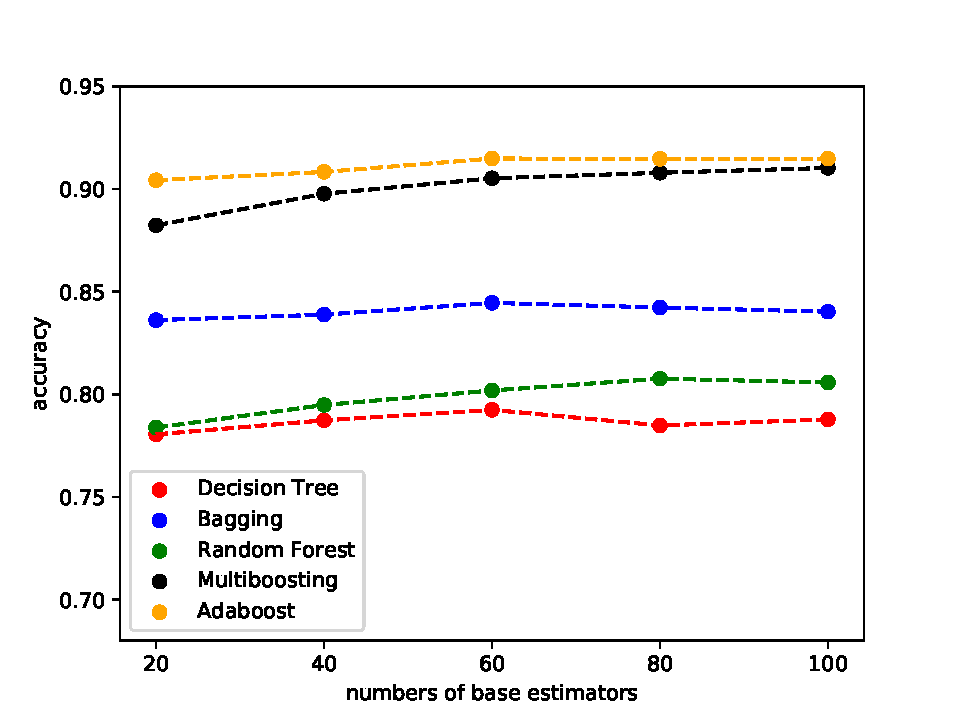
\includegraphics[width=4 in]{fig1.pdf}
  \caption{基分类器数量和正确率的关系}\label{fig1}
\end{figure}
\subsubsection{决策树最大深度}
在训练分类器的过程中,考虑到决策树的最大深度可能会带来过拟合的问题,我们考察了最大深度对分类正确率的影响。在程序中这一功能由testMax\_depth()函数实现。
\begin{table}[htbp]
 \caption{\label{tab6}决策树最大深度和准确率的关系}
 \center
 \begin{tabular}{ccccc}
  \toprule
   max\_depth &10 &15 & 20 & None  \\
  \midrule
 Decision Tree & 0.5847 & 0.7945 & 0.8371 & 0.8454 \\

 Multiboosting & 0.6300 & 0.8834 & 0.9022 & 0.8739 \\
  \bottomrule
 \end{tabular}
\end{table}
从表(\ref{tab6})中可以看到,随着决策树最大深度的增加,决策树的分类正确率不断升高,而Multiboosting算法的正确率刚开始随着最大深度的增加而增加,当不限制最大深度时,分类正确率反而下降,可以认为这时出现了Multiboosting算法退化问题。

\subsection{Multiboosting结果分析}
\begin{itemize}
  \item Multiboosting的分类正确率要大幅高于单个决策树,随机森林以及Bagging算法,比起Adaboosting略低或者相当,这可能是由于krkopt数据集的分布不均匀导致,在分析krkopt数据集时,我们发现两万八千多个样本中,有一些类别的样本数量只有几十或者几百,而一些类别的数据数量上万,因此这些数据量比较小的类别在Multiboosting 划分随机训练样本权重的过程中,很容易被Multiboosting完全忽略,而Adaboost则是首先将所有数据的置为等权重,然后增加上一轮错误数据的权重,减少正确数据的权重,使每个数据都尽可能得被照顾到,所以没有这个问题。因此我们会看到Multiboosting 算法在krkopt 数据集上比Adaboost 正确率稍微低一点的结果。另外随着基分类器数量的增加,Multiboosting 和Adaboost 的分类正确率逐渐接近,这是因为当分类器增加时,由于数据分布的不均匀导致的一部分类别的数据在随机划分下被忽略的情况得到了改善,从图\ref{fig1}可以很明显得看出这一趋势。
  \item Multiboosting的训练正确率随着基分类器个数的增加而增加,但是增加幅度会越来越小,趋于收敛,这和Adaboost相仿。因为boost类型的算法是对残差进行拟合,所以越是靠前分类器,对残差的修正越大,随着分类器数量的增加,残差会越来越小,分类器对残差的修正幅度也会越来越小,残差减小会越来越慢,趋于收敛或者在某一个值附近波动。最终的最大分类正确率会取决于样本的分布情况,以及基分类器的参数设置。
  \item Multiboosting的基分类器采用了决策树,在使用决策树的过程中,如果不限制树的最大深度,就有可能带来算法退化问题,因为Multiboosting算法在boost部分进行训练时,在不限制决策树最大深度的情况下,基分类器总是能够接近100\%的训练正确率,那么这样的话所有$\beta _t$的取值都很接近,因此Multiboosting会退化为决策树的简单组合。因此实际使用Multiboosting 时需要考虑到这一点,根据属性集对决策树设置一个合理的最大深度。
  \item Multiboosting的运行时间大于其他分类器,这是由于在fit()的过程中,算法既要完成随机划分,又要进行残差拟合,所以大大增加了算法的时间代价(当然算法缺少进行进一步的优化也是一个重要原因),所以分类正确率的提升是以训练效率为代价的。但是考虑到划分的子分类器集合进行残差拟合时可以进行并行计算,如果将程序改进成为并行程序,那么时间代价会减少很多。
\end{itemize}


\begin{appendix}

\section{关于分工}
这次大作业,李沛泽同学负责IterativeBagging算法的实现与分析工作,晁越同学负责Multiboosting算法的实现与分析以及Random Forest与Bagging的分析比较工作,李沛泽同学对Random Forest和Bagging的分析比较工作提供了一些建议和帮助。报告由二人共同撰写。
\section{关于程序的说明}
Multiboosting文件夹里的sourcefunc.py载入第三方库,multiboosting算法以及krkopt数据,multiboosting.py用来测试multiboosting算法,RFvsBG.py用来比较Random Forest和Bagging的时间代价。\par
IterativeBagging文件夹包括了IterativeBagging的分类以及回归算法。

\bibliography{514917,350132}

\end{appendix}
\end{spacing}
\end{document} 